\documentclass{article}
\usepackage[utf8]{inputenc}

\title{ProgC_V1.0}
\author{thi.schwaller444 }
\date{January 2020}
\usepackage{multicol}
\usepackage{graphicx}
\usepackage[a4paper,width=150mm,top=25mm,bottom=25mm]{geometry}
\pagestyle{myheadings}
\markright{Thierry Schwaller / https://github.com/tschwall/Zusammenfassungen}
\begin{document}
\section{Wichtige Befehle}
\textbf{Volatile:} \\
Die Variabel wird durch den Compiler nicht weg optimiert. Die Variable wird nicht in das Prozessregister gelegt.\\
\textbf{$\#$define:} \\
Die Variablen welche durch $\#$define definiert wurden werden vom Preprozessor durch ihren vorgegebenen Wert ersetzt. (Der Compiler sieht die $\#$define Varialben nie) \\
\textbf{Typedef:} \\
Reine Textersetzung. (Z.B Überall wo ein typendefiniertes Struct aufgerufen wird wird der Code der Struct durch den Compiler ergänzt) \\
\textbf{Continue:} \\
In den nächsten Schleifendurchgang springen. \\
\textbf{$\#$include}\\
\textbf{$<Name>$} $\rightarrow$ Name wird im definierten Include-Verzeichniss gesucht \\
\textbf{"Name"} $\rightarrow$ Wird im aktuellen Verzeichniss gesucht \\
\textbf{printf} $\rightarrow$ S.465
\section{Sonstiges}
\textbf{C ist casesensitive}
\textbf{Funktionsprototyp} $\rightarrow$ Deklaration einer Funktion \\
\textbf{L- und R- Werte}  $\rightarrow$ lvalue braucht immer Schreibzugriff und bei rvalue reicht Lesezugriff \\
\textbf{Globale Variablen} werden \textbf{automatisch auf 0 initialisiert} (wie globale Arrays auch) \\
\textbf{Lokale Variablen} werden beim \textbf{Aufruf des Blockes} angelegt. \\
\textbf{Funktionsprototyp} $\rightarrow$ Deklaration einer Funktion. \\
\textbf{Stub} $\rightarrow$ Entwurf eines Programm (beinhaltet alle Elemente damit das Programm ausgeführt werden kann) \\
\textbf{Bedingungsoperator} $\rightarrow$ A?B:C (if(A) then(B) else(C)) \\
\textbf{Sequenzpunkte} Bestimmter Punkt an dem alle bisherigen Nebeneffekte abgearbeitet wurden. (Ende einer if Bedingung / Zwischen $|| \&\&$ / Semikolon)\\
\textbf{const char* text} $\rightarrow$ text ist ein Pointer auf ein konstanten Char \\
\textbf{char* const text} $\rightarrow$ Der Pointer Text ist konstant\\
\textbf{Interruptvektortabelle} $\rightarrow$ Tabelle von Funktionspointern\\
\textbf{\#-Operator} $\rightarrow$ Konvertiert Argument in String \\
\textbf{\#\#-Operator} $\rightarrow$ Zeichenfolge links und echts des Operators wird zusammengezogen
\section{Nassi-Shneiderman-Diagramme}
\begin{multicols}{2}
\begin{center}
    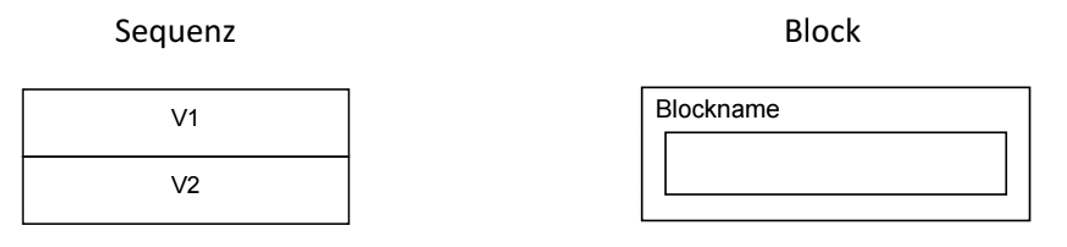
\includegraphics[width=0.4\textwidth]{Nassi1.PNG}
\end{center}
    \columnbreak
\begin{center}
    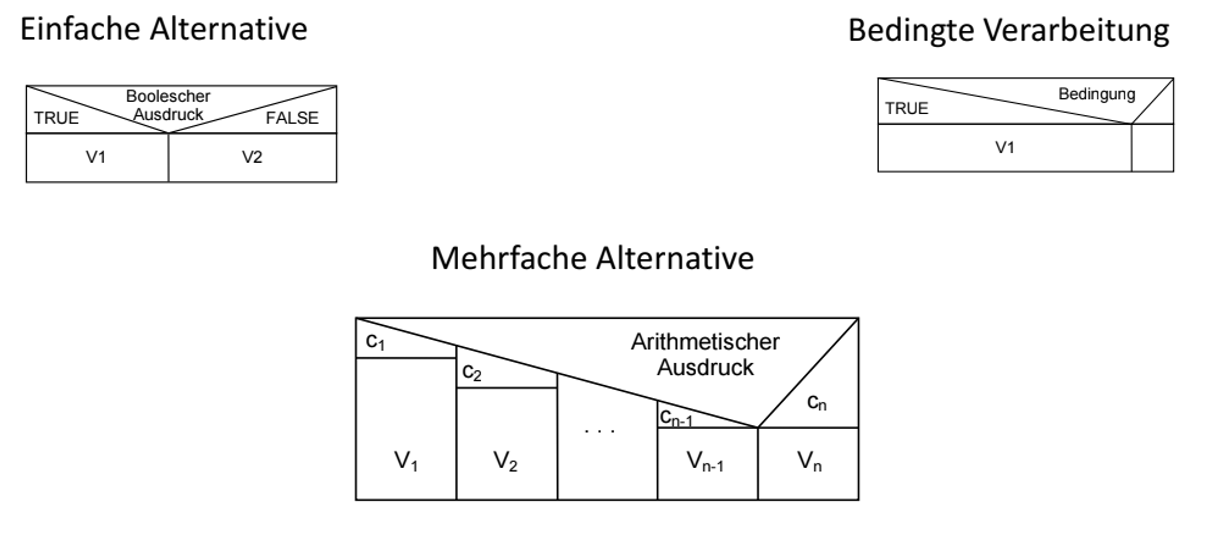
\includegraphics[width=0.4\textwidth]{Nassi2.PNG}
\end{center}
    \columnbreak
\end{multicols}
\begin{center}
    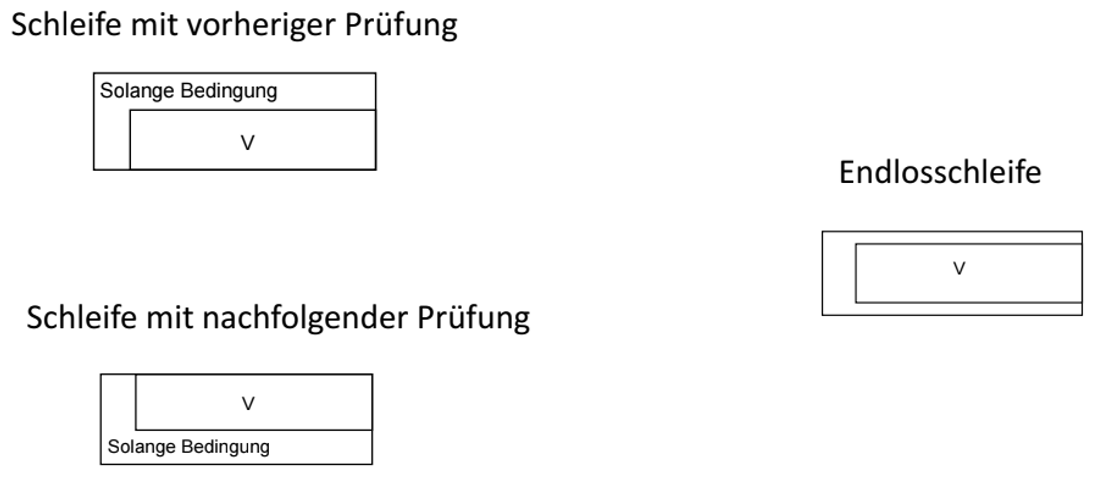
\includegraphics[width=0.4\textwidth]{Nassi3.PNG}
\end{center}
\section{Gültigkeit, Sichtbarkeit und Lebensdauer}
\textbf{Variablen sind immer so lokal wie möglich zu definieren} \\
\textbf{Gültigkeit:}\\
Eine Variabel ist dann gültig wenn sie an der genannten Stelle dem \textbf{Compiler bekannt} ist und \textbf{nicht durch eine andere Variable verdeckt} wird. \\
\textbf{Sichtbarkeit:}\\
Wird eine lokale Variable mit dem selben Namen wie eine globale Variable erstellt ist nur die lokale sichtbar. \\
\textbf{Lebensdauer:}\\
Zeit in welcher der Compiler der Variable ein Speicherplatz zu Verfügung stellt.
\section{Arbeiten mit char-Variablen}
Falls zu wenig Speicher auf einem Gerät vorhanden ist kann es vorkommen, dass das zusammenkopieren von verschiedenen Char - Arrays selber programmiert werden muss.
Dies kann mit While, for Schleifen am einfachsten realisiert werden.\\
\textbf{Falls genügend Speicherplatz vorhanden: } \\
Library $ <string.h> \rightarrow strCopy(char* dest, const char* src);$ \\
Fügt den String src ans Ende des Strings dest an. Ist allerdings dest nicht genügend gross kann dies zu Problemen führen daher wird \textbf{strnCpy() bevorzugt}\\
\textbf{Sonst: }\\
while(dest[i] = src[i]) \textbf{Weisst zu und ist true bis src[i] = Backslash 0}\\
    i++; \\
Funktionen von $<string.h>$ die mit \textbf{str} beginnen \textbf{erkennen das Backslash 0}.Funktionen die mit \textbf{mem} beginnen \textbf{nicht}. \\
Wenn \textbf{strn} verwendet wird dann kann es keinen Buffer - Overflow geben.  
\section{Pointer Basics S.163 Advanced S.320}
\begin{multicols}{2}
\begin{center}
Variable in welcher eine Adresse von einer im Speicher befindlichen Variable oder Funktion gespeichert ist. 
\end{center}
\columnbreak
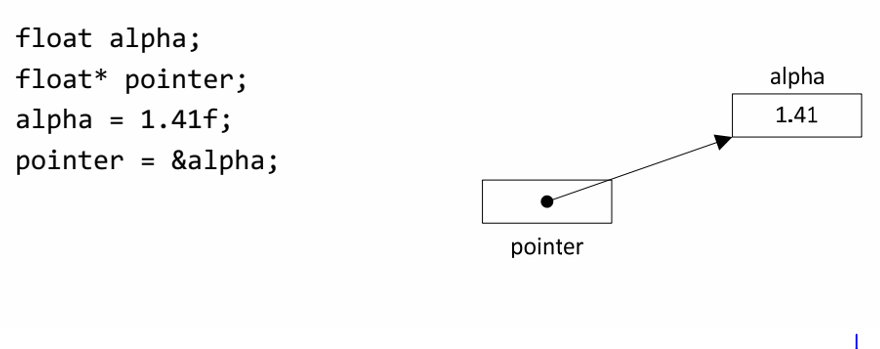
\includegraphics[width=0.5\textwidth]{Pointer_Basics.PNG}
\end{multicols}
Der \textbf{Speicherbedarf eines Pointers} ist \textbf{unabhängig vom Typ}. So gross wie die maximale Adresse.\\
Falls man ein Pointer initialisieren will muss man diesen zu einem \textbf{Nullpointer} machen. (Zeigt nicht auf Adresse 0) \\
Der Adressoperator \textbf{\&} (Referenzierungsoperator) liefert die \textbf{Adresse einer Variable}. \\
Der Inhaltsoperator \textbf{*} (Dereferenzierungsoperator liefert den Wert einer Speicherzelle.
\subsection{Array-Pointers}
Der Name eines Arrays kann als konstante Adresse des ersten Elementes (Index 0) des Arrays betrachtet werden. \\
Die Befehle $\&array[0]$ bedeutet das gleiche wie array
\subsection{Pointer auf Funktionen}
Jede Funktion befindet sich an einer definierten Adresse im Codespeicher. \\
Ein Funktionspointer wird wie folgt initialisert: \\
Rückgabetyp der Funktion (*pointer)(Datentyp der Parameter);\\
pointer = functionsname; \\
ausgabewert = pointer(parameter); \\

\section{Arrays}
sizeof(arr)/sizeof(arr[0]) gibt die Anzahl der Elemente zurück. \\

Beim Befehl \textbf{pointer + n} bewegt sich der Pointer um n * sizeof(Typ) Bytes. 
\section{Lexikalische Konventionen}
Namen dürfen aus Buchstaben, Ziffern und Underscores bestehen, allerdings darf das erste Zeichen keine Ziffer sein.
\subsection{Enumerations / Aufzählungstyp}
Anonyme Enumerations können dazu verwendet werden ganzzahlige symbolische Konstanten zu definieren. (Falls nicht ganzzahlig werden const gebraucht).
\subsection{Auswertungsreihenfolge}
\textbf{*p++} $\rightarrow$ p wird dereferenziert und danach wird der Pointer inkrementiert \\
\textbf{*++p} $\rightarrow$ p wird zuerst inkrementiert und danach dereferenziert\\
\textbf{(*p)++}$\rightarrow$ Zuerst wird *p dereferenziert und der Wert danach um 1 erhöht.\\
\textbf{int* alpha[8]} $\rightarrow$ Array von 8 int-Pointern \\
\textbf{int (*alpha)[8]} $\rightarrow$ Pointer auf ein Array mit 8 int Werten. \\
\textbf{int * (*alpha)[8]} $\rightarrow$ Pointer auf ein Array aus 8 int Pointern
\section{Bit-Operationen}
\textbf{Kann nur mit unsigned Typen durchgeführt werden.}\\
$A \& B \rightarrow$ Bitweise AND \\ 
$A | B \rightarrow$ Bitweise OR \\
$ \raisebox{-0.9ex}{\~{ }} A \rightarrow$ Bitweise NOT \\
$A \raisebox{-0.9ex}{\^{}}  B \rightarrow$ Bitweise XOR \\
$A >> n \rightarrow$ Rechts-Shift um n Bits \\
$A << n \rightarrow$ Links-Shift um n Bits
\section{Structs}
Structs können \textbf{zugewiesen} Werden (a = b) \\
\textbf{Grösse} ist nur \textbf{mit dem sizeof} Operator zu bestimmen. (Nicht zusammenzählen der einzelnen Variablen). Variablen fangen immer im nächsten Byte an dies wird \textbf{Alignment} genannt. \\
Die Adresse einer Strukturvariablen kann mit dem Adressoperator ermittelt werden.
\subsection{Zugreifen auf Strukturvariable}
\textbf{Auf Feld von einer Strukturvariablen:} \\
(Name des Structs).(Name des Feldes) \\
\textbf{Zugriff über ein Pointer auf eine Strukturvariable: } \\
(Name des Pointers)-$>$(Name des Feldes) \\
Es ist meistens effizienter einen Pointer auf eine Struct an eine Funktion zu übergeben als der Struct an sich da der Kopieraufwand grösser ist.
\subsection{Unions}
Unions sind ähnlich wie Struts allerdings ist immer nur eine Variable / Feld aktiv, dies führt dazu das man weniger Speicher braucht. Die grösse einer Union wird immer durch die grösste Variabel bestummen. \\
Da sich die Variablen den Speicherplatz teilen beeinflussen sie den Inhalt von sich gegenseitig.
\section{Iteration und Rekurstion}
\subsection{Rekursion}
Funktion enthält Abschnitt welcher sich \textbf{selbst aufruft}. Alle noch auszuführende Befehle werden im Stack gespeichert. (Kann zu einem Stack-Overflow führen)
\subsection{Iteration}
Funktion enthält Abschnitt welcher mehrfach durchlaufen wird. \textbf{Jede Funktion} ist \textbf{iterativ} definierbar. In der Praxis wird immer die Iterative Form gebraucht.
\section{Speicherklassen}
Vier verschiedene Speicherbereiche
\begin{itemize}
    \item Code\\
    Zugriff: lesen, ausführen (im Flash EPROM oder im RAM) \\
    Programm im Maschinencode und eventuell Konstanten (meist grosse Konstante Arrays)
    \item Datensegment / Stack / Heap \\
    Zugriff: lesen und schreiben (im RAM (evtl. Register))
    \subitem Datensegment \\
    Globale Variablen, static Variablen
    \subitem Stack \\
    Lokale Variablen, Parameter einer Funktion, Rücksprungadressen
    \subitem Heap \\
    Dynamische Variablen (Speicherplatz erst zu Laufzeit gefordert)
\end{itemize}
\section{Arbeiten in grossen Projekten}
\textbf{Gültigkeit von Variablen o.Ä möglichst klein halten} (Information Hiding)
\subsection{Programm aus mehreren Dateien}
Zuerst müssen alle Sourcedateien compiliert werden und danach werden sie zusammengelinkt und eine einzige auszuführende Datei entsteht. (Wird Buildprozess genannt). \\
\textbf{Interne Bindungen} $\rightarrow$ Symbole welche nur in einer Übersetzungseinheit vorkommen \\
\textbf{Externe Bindungen} $\rightarrow$ Symbole werde in mehreren Übersetzungeinheiten gebraucht (Werde über Linker untereinander bekannt gemacht). \\
\textbf{Speicherklasse "extern":} \\
Eine externe Variable kann nur \textbf{in einer Datei definiert werden (ohne extern)}. In den anderen wird sie mit \textbf{extern deklariert (bekannt gemacht)}. \\ 
Der Speicherplatz wird nur einmal benötigt \\
\textbf{Speicherklasse "static":} \\
Der Wert einer Static Variable bleibt erhalten nachdem die Funktion beendet wurde. Nur in definierter Datei sichtbar
\section{Preprocessor}
Output des Preprocessors wird dem eigentlichen Compiler übergeben
$<\#$ - Befehle werden durch den Preprocessor ausgeführt.Arbeitet Zeilerorientiert
\section{Input / Output Kapitel 16.8}
\textbf{Dateienzugriff über Filepointer:} \\
Mit einem Filepointer kann eine Datei mit dem C- Code verknüpft werden.\\
FILE * fp = fopen("test.dat", "rw") \\
Es gibt drei vordefinierte Standardkanäle (Filepointer): 
\begin{itemize}
    \item Standardeingabe \textbf{stdin} \\
    Tastatur
    \item Standardausgabe \textbf{stdout} \\
    Konsole
    \item Standardfehlerausgabe \textbf{stderr} \\
    Oft die Konsole
\end{itemize}
\subsection{Umlenkung}
Mit einer Umlenkung kann die Standardaus- und eingabe umgeleitet werden, zum Beispiel in ein Textfile. \\
Dies kann mit den Operatoren $< \textrm{(Eingabe) und } > \textrm{(Ausgabe)}$ gemacht werden. 
\section{Kommandozeilenparameter}
Ziel ist die Parameter für ein Programm gerade beim Aufrufen der Funktion mitzugeben. \\
Dafür wird \textbf{int main} angepasst und zwar wie folgt: \\
int main(int argc, char* argv[]);
\textbf{argc} $\rightarrow$ Argumentcounter
\textbf{argv} $\rightarrow$ Argumentvektor (argv[0] beinhaltet immer den Namen des Programms)
\end{document}
